% Koma class
\documentclass[a4paper, oneside]{scrartcl}   

\usepackage{a4wide}
\usepackage{german}
\usepackage{amssymb}
\usepackage{tikz}
\usepackage[latin1]{inputenc}

%------------------
% language = english
\usepackage[english]{babel}	% Umlaute mit \"u
\usepackage[latin1]{inputenc}

% margins + Kopf- und Fu�zeilen
\usepackage[left = 2.5cm, right = 2.5cm, top = 2cm, bottom = 3cm]{geometry}
\usepackage{scrpage2} 
\pagestyle{scrheadings}
\clearscrheadfoot
\rehead{\headmark}
\lehead{\pagemark}
\lohead{\headmark}
\rohead{\pagemark} 


% math
\usepackage{amsmath}

% figures
\usepackage{graphicx}


% section-Zaehler wird neu gesetzt:
\setcounter{section}{1}
%------------------
\author{Sascha Meiers, Martin Seeger}
\title{Exercise 1, Discrete Mathematics for Bioinformatics}
\date{Winter term 2011/2012}


\begin{document}
\maketitle



%---------------------------------------------------------------------------------------------------

\subsection{MST Approximation}

a)

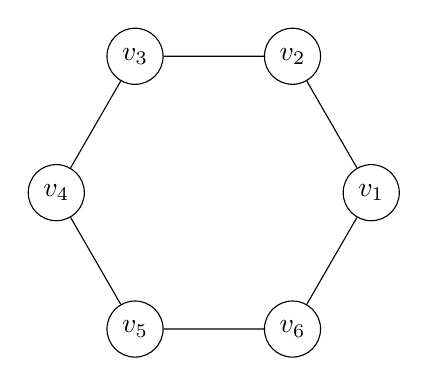
\begin{tikzpicture}
% Default actions for each node
\tikzstyle{every node}=[draw, shape=circle];
% Define and draw five nodes
\node (v1) at (0:2) {$v_1$};
\node (v2) at (60:2) {$v_2$};
\node (v3) at (120:2) {$v_3$};
\node (v4) at (180:2) {$v_4$};
\node (v5) at (240:2) {$v_5$};
\node (v6) at (300:2) {$v_6$};
% Draw radial edges
\draw (v1) -- (v2) (v2) -- (v3)
(v3) -- (v4) (v4) -- (v5)
(v5) -- (v6) (v6) -- (v1);
\end{tikzpicture}

b)

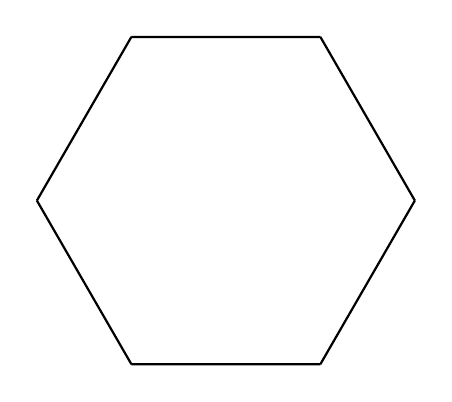
\begin{tikzpicture}[thick,scale=0.8]%
    \draw \foreach \x in {0,60,...,300} {
        (\x:3) node{} -- (\x+60:3)
};
\end{tikzpicture}

\subsection{Landau Symbols}

\renewcommand{\labelenumi}{\alph{enumi})}
\begin{enumerate}
\item Let $k, l \in \mathbb{Z}$, $k > l$. $f = o(g)$ holds iff 
\begin{equation}
\lim_{n\rightarrow \infty} \left|\frac{f(n)}{g(n)}\right| = 0. 
\end{equation}
In our case, 
\begin{equation}
\lim_{n\rightarrow \infty} \left|\frac{f(n)}{g(n)}\right| = \lim_{n\rightarrow
\infty} \left|\frac{n^l}{n^k}\right| = \lim_{n\rightarrow
\infty} \left|\frac{1}{n^{k-l}}\right| = 0,
\end{equation}
whence it follows that $n^l=o(n^k)$.$\square$

\item Let $k, l \in \mathbb{N}$, $k > l$. In general, $f=\Theta(g)$ iff
$f=O(g)$ and $g=O(f)$. We use the definition $f=O(g)$ iff
\begin{equation}
0 \leq \limsup_{n\rightarrow \infty} \left|\frac{f(n)}{g(n)}\right| < \infty. 
\end{equation}
In our case, 
\begin{equation}
\limsup_{n\rightarrow \infty} \left|\frac{n^k+n^l}{n^k}\right| =
\limsup_{n\rightarrow \infty} \left|1 + \frac{1}{n^{k-l}}\right| = 1,
\end{equation}
and
\begin{equation}
\limsup_{n\rightarrow \infty} \left|\frac{n^k}{n^k+n^l}\right| =
\limsup_{n\rightarrow \infty} \left|1 - \frac{n^l}{n^k+n^l}\right| =
\limsup_{n\rightarrow \infty} \left|1 - \frac{1}{n^{k-l}+1}\right| =
1.\square
\end{equation}
 
\item Counterexample: $f(n)=2^{cn}$ with $c>1$ is clearly $2^{O(n)}$. However, 
\begin{equation}
\limsup_{n\rightarrow \infty} \left|\frac{2^{cn}}{2^{n}}\right| =
\limsup_{n\rightarrow \infty} 2^{(c-1)n} = \infty,
\end{equation}
hence $f \neq O(2^n)$.$\square$
\end{enumerate}

\subsection{Amortized Analysis}

x

\subsection{Analysis of \textsc{Select} algorithm}

The \textsc{Select} algorithm is given a list $A$ of $n$ numbers (or elements of a completely ordered universe) 
and a rank $k\leq n$. It returns the $k$-th smallest element of $A$.

The deterministic \textsc{Select} algorithm guarantees a worst-case complexity of $\mathcal{O}(n)$ by smartly choosing a Pivot element. 
This is achieved by dividing the elements of the list into groups of 5 
(in general $r$, meaning \textit{row} as related to the figure) and calculating the medians of each group in constant time 
(since a group contains only constant many elements). The same routine is used recursively to determine the median of these medians. 
Finally the whole list is split up like in Quicksort, using the median of medians for Pivot element, and the search is continued in 
only one of both parts depending on $k$. As is shown in the additional material, splitting at this point drops always enough elements for the runtime to be linear in $n$. Here we want to investigate wether the linear-time property holds for other values of $r$, too.

The runtime of the \textsc{Select} algorithm can be written recursively as 
\[ T(n) = T(\left\lceil \frac{n}{r} \right\rceil ) + T(g(n)) + an \]
\begin{itemize}
\item $T(\left\lceil \frac{n}{r} \right\rceil)$ is the runtime for the recursive call of \textsc{Select} in order to 
compute the median of medians. 
\item $c\cdot n$ is the runtime of dividing the list into groups of $r$, finding their 
medians (which works in $\mathcal{O}(r\; log\; r)$, i.e. in $\mathcal{O}(1)$ for each group) and finally splitting up the list.
\item $T(g(n))$ is the runtime of the recursive call of \textsc{Select} on a smaller list. $g(n)$ is an upper bound for the 
length of this list and by association the key variant in enabling a linear overall runtime. For $r=5$ we've seen that 
$g(n) \leq \frac{7}{10} n + 6 $.
\end{itemize}

\begin{figure}
\centering
\includegraphics[width=10cm]{deterministic_select.pdf}
\end{figure}

The figure shows the partial ordering we obtain by determining the median of medians. At least the elements in the lower 
right box are larger than or equal to the Pivot element $x$, but there can be more in the upper right or lower left quarter. 
On the other side there is at least the upper left quarter of elements that are lower than or equal to $x$. Let's assume $r$ 
to be odd (since we then can clearly determine a median). Then the lower right quarter consists of 
$\left\lceil \frac{n}{2r} \right\rceil$ columns with each $\frac{r+1}{2}$ elements except for the last columns, wich contains 
at least one element. So we will not count the last column and we will also deduct the column of $x$ itself (the same is done in the additional material). So the maximum number of elements in the next recursive call for an odd number $r$ is

\begin{align*}
g(n) &\leq n - \left( \left\lceil \frac{n}{2r} \right\rceil -2\right) \cdot \frac{r+1}{2}\\
     &\leq n - \left( \frac{n}{2r} -2\right) \cdot \frac{r+1}{2}\\
     &\leq (0.75 - \frac{1}{4r})\cdot n +(r+1) .
\end{align*}
Due to monotonicity of the runtime function, $T(n)$ is now determined by
\begin{align*}
T(n) &\leq T\left( \frac{n}{r} +1 \right) + T\left( (0.75 - \frac{1}{4r})\cdot n +(r+1) \right) + an 
\end{align*}
Now assume that $T(n) \leq c\cdot n$ for large $n$ and a constant factor $c$. Then we have
\begin{align*}
T(n) &\leq c\cdot \left( \frac{n}{r} \right) +c + c\cdot \left( (0.75 - \frac{1}{4r})\cdot n +(r+1) \right) + an \\
     & =    cn \left(\frac{1}{r} + 0.75 - \frac{1}{4r}\right) + an + (r+2)c \\
     & = cn - cn \left(\frac{r-3}{4r}\right) + an + (r+2)c
\end{align*}
In order to complete the proof, we have to show that this recursively defined runtime is at most $cn$, too. 
This depends on the term after $cn$: If it is at most zero, the runtime is linear.
We have to differ two cases: If $r\leq 3$, then there are only positive addends in the term and the inequality obviously does not hold. 
Otherwise, if $r>3$, the fraction $\frac{r-3}{4r}$ is larger than zero but less than one and we can find the factor $c$ as needed: 
\begin{align*}
- cn \left(\frac{r-3}{4r}\right) + an + (r+2)c &\leq 0 \\
c \left( -n\frac{r-3}{4r} +r +2 \right) &\leq -an \\
c &\geq \frac{an} { n\frac{r-3}{4r} -r -2 }		\qquad \| \; \text{for } n > r+2
\end{align*}
This inequality can be solved for any $r>3$, if $n$ is chosen large enough (for example $n> 2(r+2)$). If we choose $r=5$, 
we can exactly reproduce the example from the additional material:
\begin{align*}
c &\geq \frac{an} { n\frac{5-3}{4\cdot 5} -5 -2 }		& \| \; \text{for } n > 5+2 \\
c &\geq \frac{10an} {n - 70}  & \\ 
c &\geq 20a 					& \| \; \text{for } n>140\text{, because } \frac{n}{n-70}\leq 2
\end{align*}
Finally we found a constant factors $c$ (which of course depends on the factor $a$ for splitting the list etc.) such that the overall runtime is linear. During the derivation we found that the linear runtime only works for $r>3$, which answers the initial question.





\end{document}


\begin{document}
\maketitle

%\section{Title}

\end{document}